% =====================================================================
%  Encounter risk classification on Synthea data
%  Compile with:  latexmk -pdf report.tex      (or upload the folder to Overleaf)
% =====================================================================
\documentclass[11pt,a4paper]{article}

% ---------- Encoding, fonts, layout ----------
\usepackage[utf8]{inputenc}
\usepackage[T1]{fontenc}
\usepackage[sc]{mathpazo}
\linespread{1.06}
\usepackage[a4paper,margin=2.6cm]{geometry}
\usepackage{microtype}

% ---------- Math, tables, figures ----------
\usepackage{amsmath,amssymb}
\usepackage{booktabs}
\usepackage{multirow}
\usepackage{array}
\usepackage{graphicx}
\usepackage{float}
\usepackage{caption}
\usepackage{subcaption}
\usepackage{xcolor}
\usepackage{enumitem}
\usepackage{tikz}
\usetikzlibrary{positioning,arrows.meta,shapes.misc}

% ---------- Colours and links ----------
\definecolor{accent}{HTML}{2A78D6}
\definecolor{accent2}{HTML}{EB6834}
\definecolor{rowgrey}{HTML}{F3F5F8}
\definecolor{codegrey}{HTML}{555555}
\usepackage[colorlinks=true,linkcolor=accent,citecolor=accent,urlcolor=accent]{hyperref}

\captionsetup{font=small,labelfont={bf,color=accent},width=0.92\textwidth}
\setlist{nosep,leftmargin=*}
\graphicspath{{figures/}}
\setlength{\emergencystretch}{3em}

% ---------- Helpers ----------
\newcommand{\code}[1]{\texttt{\textcolor{codegrey}{#1}}}
\newcommand{\best}[1]{\textbf{\textcolor{accent}{#1}}}
\newcommand{\sect}[1]{\section{#1}}
\newcolumntype{R}{>{\raggedleft\arraybackslash}p{1.45cm}}

% ---------- Title ----------
\title{\vspace{-1.2cm}
  {\LARGE\bfseries Predicting the Risk Class of a Hospital Encounter}\\[0.4em]
  {\large From raw Synthea records to a comparison of six classifiers}\vspace{-0.2cm}}
\author{Hospital prediction project --- Intelligence Artificielle, S4a}
\date{November 2026}

\begin{document}
\maketitle

\begin{abstract}
\noindent
This report documents a complete machine-learning pipeline built on synthetic electronic health
records generated by Synthea. Twelve raw CSV tables were consolidated into a single table of
103{,}189 hospital encounters, one row per visit, each described by 69 attributes known
\emph{before} the visit started. A four-level risk label (Low, Medium, High, Critical) was derived
from the encounter type, its relative cost and 30-day mortality. After preprocessing (encoding,
missing-value handling and imputation), six classical classifiers were tuned by cross-validation
and compared on a stratified held-out test set of 20{,}638 encounters. Histogram-based gradient
boosting obtained the best accuracy (0.857) and macro-F1 (0.479), and recovered 51\,\% of the
Critical encounters, whereas Gaussian Naive Bayes collapsed to the majority class. The main
difficulty of the task is the strong class imbalance: 84\,\% of encounters are Low risk, and the
Medium and High classes remain hard to separate from it.
\end{abstract}

\tableofcontents
\vspace{0.5em}
\hrule
\vspace{1em}

% =====================================================================
\sect{Introduction}
% =====================================================================

Emergency departments and hospitals need to anticipate which incoming patients are likely to
require heavy care. The goal of this project is to predict, for a given encounter and using only
the patient's history \emph{prior} to that encounter, a \textbf{risk class} on a four-level scale.
Such a model could help triage, staffing or bed-management decisions.

The work was organised in four steps, each materialised by one script or notebook
(Figure~\ref{fig:pipeline}):

\begin{enumerate}[itemsep=2pt]
  \item \textbf{Dataset construction} (\code{build\_dataset.py}): merge the Synthea CSV tables
        into one encounter-level table and define the target.
  \item \textbf{Preprocessing} (\code{preprocessing.ipynb}): encode categorical attributes,
        handle missing values and prepare a purely numeric matrix.
  \item \textbf{Training} (\code{training.ipynb}): split the data, tune six classifiers with
        cross-validation and persist the fitted models.
  \item \textbf{Evaluation} (\code{evaluation.ipynb}): score every model on the same held-out
        test set and compare them.
\end{enumerate}

\begin{figure}[H]
\centering
\resizebox{\textwidth}{!}{%
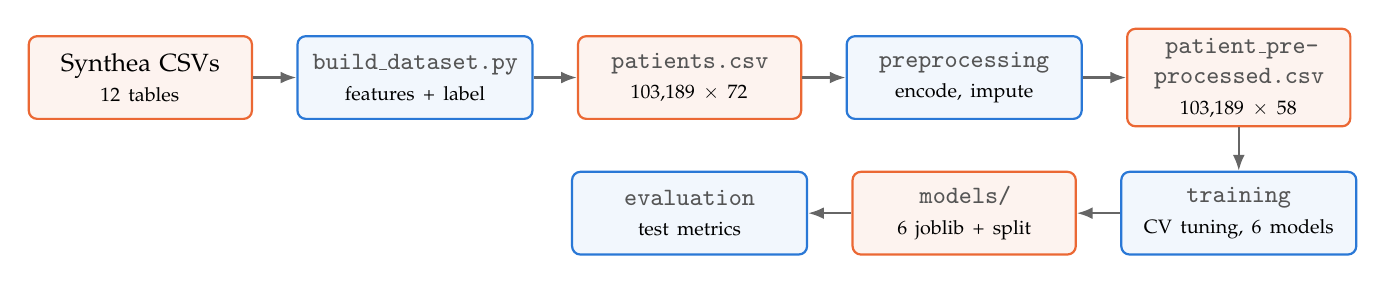
\begin{tikzpicture}[
  node distance=0.55cm and 0.55cm,
  box/.style={draw=accent, thick, rounded corners=3pt, fill=accent!6, minimum height=1.05cm,
              text width=2.75cm, align=center, font=\small},
  data/.style={draw=accent2, thick, rounded corners=3pt, fill=accent2!8, minimum height=1.05cm,
               text width=2.6cm, align=center, font=\small},
  arr/.style={-{Latex[length=2mm]}, thick, color=black!60}
]
  \node[data] (raw)  {Synthea CSVs\\ \scriptsize 12 tables};
  \node[box,  right=of raw]  (build) {\code{build\_dataset.py}\\ \scriptsize features + label};
  \node[data, right=of build] (ds)   {\code{patients.csv}\\ \scriptsize 103{,}189 $\times$ 72};
  \node[box,  right=of ds]   (pre)  {\code{preprocessing}\\ \scriptsize encode, impute};
  \node[data, right=of pre]  (pp)   {\code{patient\_pre-}\\\code{processed.csv}\\ \scriptsize 103{,}189 $\times$ 58};
  \node[box,  below=of pp]   (train) {\code{training}\\ \scriptsize CV tuning, 6 models};
  \node[data, left=of train] (models) {\code{models/}\\ \scriptsize 6 joblib + split};
  \node[box,  left=of models] (eval) {\code{evaluation}\\ \scriptsize test metrics};
  \draw[arr] (raw) -- (build);
  \draw[arr] (build) -- (ds);
  \draw[arr] (ds) -- (pre);
  \draw[arr] (pre) -- (pp);
  \draw[arr] (pp) -- (train);
  \draw[arr] (train) -- (models);
  \draw[arr] (models) -- (eval);
\end{tikzpicture}}
\caption{Overview of the pipeline. Orange boxes are data artefacts, blue boxes are code.}
\label{fig:pipeline}
\end{figure}

% =====================================================================
\sect{Source data}
% =====================================================================

The data come from \textbf{Synthea}, an open-source generator of realistic but entirely synthetic
patient histories. A Synthea export is a set of CSV files, each describing one kind of clinical
event and linked by patient and encounter identifiers. Table~\ref{tab:tables} lists the tables
used here and what each one contributed.

\begin{table}[H]
\centering\small
\caption{Synthea tables consumed by \code{build\_dataset.py}.}
\label{tab:tables}
\begin{tabular}{@{}lp{4.1cm}p{7.6cm}@{}}
\toprule
\textbf{Table} & \textbf{Key column(s)} & \textbf{Used for} \\
\midrule
\code{encounters}      & \code{START}, \code{ENCOUNTERCLASS}, \code{TOTAL\_CLAIM\_COST} & The sampling unit (one row per visit) and the target label \\
\code{patients}        & \code{BIRTHDATE}, \code{DEATHDATE}, demographics & Age, gender, race, ethnicity, income; 30-day mortality for the label \\
\code{conditions}      & \code{START}, \code{DESCRIPTION} & Count of prior diagnoses; ten binary risk-factor flags \\
\code{medications}     & \code{START} & Count of prior prescriptions \\
\code{procedures}      & \code{START} & Count of prior procedures \\
\code{immunizations}   & \code{DATE}  & Count of prior vaccinations \\
\code{allergies}       & \code{START} & Count of prior allergy records \\
\code{careplans}       & \code{START} & Count of prior care plans \\
\code{imaging\_studies} & \code{DATE} & Count of prior imaging studies \\
\code{devices}         & \code{START} & Count of prior medical devices \\
\code{observations}    & \code{DATE}, \code{DESCRIPTION}, \code{VALUE} & Latest known value of 44 numeric measurements (vitals, labs, questionnaires) \\
\bottomrule
\end{tabular}
\end{table}

% =====================================================================
\sect{Dataset construction}
% =====================================================================

\subsection{Sampling unit and temporal discipline}

Each \textbf{encounter} is one sample. The central design rule is that every feature must be
computable from information available \emph{strictly before} the day of the encounter. This avoids
target leakage and makes the task a genuine prediction problem: at admission time, the hospital
knows the patient's past, not what the current visit will turn into.

Encounters are sorted chronologically. For every event table, a helper function
(\code{prior\_counts}) merges the encounter timestamps with the event timestamps, sorts them per
patient, and uses a cumulative sum to count how many events happened before each encounter day.
This runs in a single pass and scales to the full history of every patient.

\subsection{Target: the risk score and risk class}

Synthea does not provide a notion of risk, so a label was engineered from three signals of visit
severity. For an encounter $e$ of class $c$ (wellness, ambulatory, outpatient, urgent care,
emergency or inpatient):

\begin{equation}
  \text{risk\_score}(e) \;=\; \operatorname{clip}_{[0,1]}\Big(
     \underbrace{b_c}_{\text{visit type}}
     \;+\; 0.15 \cdot \underbrace{\text{cost\_pct}(e)}_{\text{relative cost}}
     \;+\; 0.25 \cdot \underbrace{\text{died}_{30}(e)}_{\text{mortality}}
  \Big)
  \label{eq:score}
\end{equation}

\noindent where
\begin{itemize}[itemsep=2pt]
  \item $b_c$ is a base severity for the visit type:
        wellness 0.05, ambulatory 0.10, outpatient 0.15, urgent care 0.35, emergency 0.60,
        inpatient 0.70;
  \item $\text{cost\_pct}(e) \in [0,1]$ is the percentile rank of the claim cost
        \emph{within encounters of the same class}, so an unusually expensive outpatient visit
        scores higher than a routine one;
  \item $\text{died}_{30}(e) \in \{0,1\}$ indicates that the patient died within 30 days after the
        encounter.
\end{itemize}

The continuous score is then binned into four classes, which form the classification target:

\begin{center}\small
\begin{tabular}{@{}lcrr@{}}
\toprule
\textbf{Class} & \textbf{Score interval} & \textbf{Encounters} & \textbf{Share} \\
\midrule
Low      & $(0.00,\,0.25]$ & 86{,}918 & 84.2\,\% \\
Medium   & $(0.25,\,0.50]$ & 10{,}185 &  9.9\,\% \\
High     & $(0.50,\,0.75]$ &  4{,}395 &  4.3\,\% \\
Critical & $(0.75,\,1.00]$ &  1{,}691 &  1.6\,\% \\
\bottomrule
\end{tabular}
\end{center}

The distribution is heavily skewed: more than five out of six encounters are Low risk, and the
Critical class represents fewer than two encounters in a hundred. This imbalance shapes every later
decision and result. Note that none of the three ingredients of the label (encounter class, cost,
death) is used as a feature.

\subsection{Features}

The 69 raw attributes fall into four families (Table~\ref{tab:features}; the full list is in
Appendix~\ref{app:features}).

\begin{table}[H]
\centering\small
\caption{Feature families produced by \code{build\_dataset.py}.}
\label{tab:features}
\begin{tabular}{@{}lcp{8.6cm}@{}}
\toprule
\textbf{Family} & \textbf{\#} & \textbf{Content} \\
\midrule
Demographics & 5 & \code{age} at the encounter (years, fractional), \code{INCOME}, \code{GENDER}, \code{RACE}, \code{ETHNICITY} \\
History counts (\code{prior\_*}) & 10 & Number of previous visits, previous \emph{urgent} visits (urgent care, emergency, inpatient), conditions, medications, procedures, immunizations, allergies, care plans, imaging studies and devices \\
Risk-factor flags (\code{rf\_*}) & 10 & Binary indicators built by regex matching on condition descriptions: hypertension, diabetes, heart disease, COPD, obesity, smoking, stroke, chronic kidney disease, cancer, asthma \\
Observations (\code{obs\_*}) & 44 & Most recent numeric value of each measurement recorded before the encounter (vitals, blood chemistry, blood count, lipid panel, questionnaires such as PHQ-2, GAD-7, AUDIT-C) \\
\bottomrule
\end{tabular}
\end{table}

\paragraph{Observations.}
The \code{observations} table is long-format (one row per measurement). Only numeric
measurements were kept, and only those recorded for at least 20\,\% of the patients, in order to
discard rare tests. The table was pivoted to one column per measurement, values were
forward-filled per patient so that each row carries the \emph{last known} value of every
measurement, and the result was joined to the encounters with a backward as-of merge
(\code{pd.merge\_asof}) that only matches observations strictly earlier than the encounter.
Encounters with no prior observation at all were dropped.

\paragraph{Result.}
The script produced a table of \textbf{103{,}189 encounters} belonging to 5{,}757 distinct
patients, with 72 columns: the patient identifier, 69 features, the continuous
\code{risk\_score} and the categorical \code{risk\_class}. Patients are between 0 and 111 years
old (median 56), and the most frequent risk-factor flags are diabetes or prediabetes (63\,\%),
obesity (60\,\%), hypertension (47\,\%) and chronic kidney disease (40\,\%).

% =====================================================================
\sect{Preprocessing}
% =====================================================================

The preprocessing notebook turns the raw table into a fully numeric matrix without missing
values. Each step is listed below in the order it was applied.

\begin{enumerate}[itemsep=3pt]
  \item \textbf{Age decomposition.} The fractional age was split into two integer columns,
        \code{age\_years} and \code{age\_months} ($0$--$11$), which keeps the same information in a
        form that is easier to interpret.
  \item \textbf{Gender.} One-hot encoded into \code{gender\_m} and \code{gender\_f}
        (51{,}702 male and 51{,}487 female rows, an almost perfect balance).
  \item \textbf{Race.} Ordinal-encoded into a single integer column \code{race} with the mapping
        white\,=\,0, black\,=\,1, asian\,=\,2, other\,=\,3, hawaiian\,=\,4, native\,=\,5
        (white is 80\,\% of rows).
  \item \textbf{Ethnicity.} Reduced to one binary flag \code{is\_hispanic} (11\,\% positive).
  \item \textbf{Missing-value audit.} Only the observation columns had gaps; demographics,
        counts and flags were complete by construction. The missing rate of every column was
        saved to \code{data/output/patient\_missing\_columns.csv}.
  \item \textbf{Column pruning.} The 16 observation columns with more than 50\,\% missing values
        were dropped (Table~\ref{tab:dropped}). These are essentially the complete blood count
        panel, body temperature, the paediatric BMI percentile and three screening questionnaires.
  \item \textbf{Imputation.} The remaining observation gaps were filled with the \textbf{median
        of the patient's age group}, using nine clinically meaningful age bands
        ($\le 1$, 1--5, 5--12, 12--18, 18--30, 30--45, 45--65, 65--80, $>80$ years). A global
        median was used as a fallback. Vitals and lab values vary strongly with age, so this is
        far more faithful than a single global median. After this step no missing value remains.
  \item \textbf{Label encoding.} \code{risk\_class} was mapped to integers:
        Low\,=\,0, Medium\,=\,1, High\,=\,2, Critical\,=\,3.
\end{enumerate}

\begin{table}[H]
\centering\small
\caption{Observation columns removed because more than half of their values were missing.}
\label{tab:dropped}
\begin{tabular}{@{}p{11.5cm}r@{}}
\toprule
\textbf{Measurement} & \textbf{Missing} \\
\midrule
Body temperature & 89.2\,\% \\
BMI percentile per age and sex & 88.6\,\% \\
Platelet mean volume; platelet distribution width & 67.8\,\% \\
Hematocrit & 64.4\,\% \\
Erythrocytes, erythrocyte distribution width, hemoglobin, leukocytes, MCH, MCHC, MCV, platelets & 63.1\,\% \\
DAST-10 total score & 56.2\,\% \\
AUDIT-C total score & 56.1\,\% \\
HARK total score & 53.1\,\% \\
\bottomrule
\end{tabular}
\end{table}

The output, \code{patient\_preprocessed.csv}, has 103{,}189 rows and 58 columns:
the patient identifier, \textbf{55 numeric features} (1 income, 10 history counts, 10 flags,
28 observations, 6 encoded demographics) and the two targets.

% =====================================================================
\sect{Experimental protocol}
% =====================================================================

\subsection{Train / test split}

The feature matrix $X$ (55 columns) and the label $y = $ \code{risk\_class} were split
\textbf{once}, stratified on $y$, with 80\,\% for training and 20\,\% for testing
(random seed 156\,543\,894). The test indices were written to \code{models/split.json} so that the
evaluation notebook scores every model on exactly the same rows.

\begin{center}\small
\begin{tabular}{@{}lrrrrr@{}}
\toprule
 & \textbf{Low} & \textbf{Medium} & \textbf{High} & \textbf{Critical} & \textbf{Total} \\
\midrule
Training set & 69{,}534 & 8{,}148 & 3{,}516 & 1{,}353 & 82{,}551 \\
Test set     & 17{,}384 & 2{,}037 &   879 &   338 & 20{,}638 \\
\bottomrule
\end{tabular}
\end{center}

\subsection{Hyper-parameter tuning}

Tuning every model on 82{,}551 rows would take hours for the slower algorithms. The protocol
therefore separates \emph{searching} from \emph{fitting}:

\begin{enumerate}[itemsep=2pt]
  \item A stratified subsample of \textbf{20{,}000 training rows} is used for all searches.
  \item Each candidate configuration is scored by \textbf{3-fold stratified cross-validation}
        on that subsample. Four metrics are recorded for every fold: accuracy, macro-F1,
        macro-recall and the recall of the Critical class.
  \item The configuration with the best mean CV \textbf{accuracy} is selected
        (the notebook makes the tuning metric a single constant; see the discussion in
        Section~\ref{sec:discussion}).
  \item The winning configuration is refitted on the \textbf{full training set}, and the
        fitted estimator is saved with \code{joblib}.
\end{enumerate}

Small grids are searched exhaustively (\code{GridSearchCV}); large ones are sampled with
\code{RandomizedSearchCV}. The whole training notebook runs in about 6 minutes.

\subsection{Models and search spaces}

Six classifiers covering distinct inductive biases were compared. Distance-based and linear
models are wrapped in a pipeline with a \code{StandardScaler}; tree ensembles are scale-invariant
and use the raw features.

\begin{table}[H]
\centering\footnotesize
\caption{Models, search spaces and selected hyper-parameters.}
\label{tab:models}
\begin{tabular}{@{}p{2.6cm}p{5.7cm}p{4.3cm}r@{}}
\toprule
\textbf{Model} & \textbf{Search space} & \textbf{Selected} & \textbf{Fits} \\
\midrule
KNN (scaled) &
  $k \in \{1,\dots,50\}$; weights uniform / distance &
  $k=17$, uniform & 100 (grid) \\
Logistic regression (scaled) &
  $C \in \{0.01, 0.1, 1, 10, 100\}$; class weight none / balanced &
  $C=0.1$, no weighting & 10 (grid) \\
Random forest &
  trees $\{100,200,300,500\}$; depth $\{\infty,10,20,30\}$; min split $\{2,5,10\}$; min leaf $\{1,2,4\}$; max features $\{\sqrt{p},\log_2 p, 0.5\}$; criterion gini / entropy; class weight none / balanced / balanced subsample &
  100 trees, depth 10, min leaf 2, $\sqrt{p}$ features, entropy, no weighting & 30 (random) \\
SVM, RBF kernel (scaled) &
  $C \in \{0.3,1,3,10,30\}$; $\gamma \in \{\text{scale},0.01,0.03,0.1\}$; class weight none / balanced &
  $C=3$, $\gamma=0.01$, no weighting & 16 (random) \\
Gaussian naive Bayes &
  variance smoothing $\in \{10^{-12},\dots,10^{0}\}$ (13 log-spaced values) &
  smoothing $=1.0$ & 13 (grid) \\
Hist.\ gradient boosting &
  learning rate $\{0.03,0.05,0.1,0.2\}$; iterations $\{100,200,400\}$; max leaves $\{15,31,63\}$; min leaf $\{10,20,50\}$; $\ell_2$ $\{0,0.1,1\}$; class weight none / balanced &
  rate 0.03, 400 iterations, 31 leaves, min leaf 20, $\ell_2=0.1$, no weighting & 20 (random) \\
\bottomrule
\end{tabular}
\end{table}

Two practical constraints are worth noting. The RBF SVM has roughly quadratic training cost, so
its final model was fitted on a stratified subsample of 40{,}000 training rows (51 s) rather than
the full set; the linear kernel was skipped because logistic regression already covers the linear
case. Every other model was refitted on all 82{,}551 rows.

\begin{figure}[H]
\centering
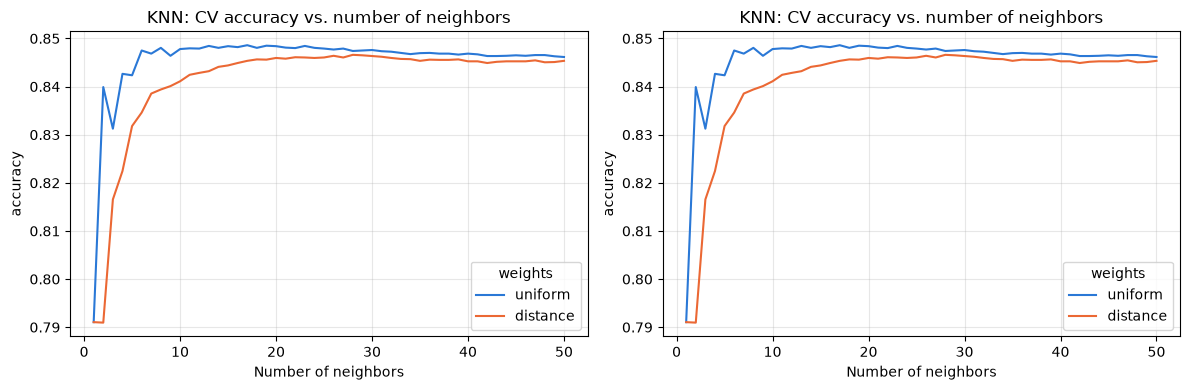
\includegraphics[width=\textwidth]{knn_tuning}
\caption{KNN tuning curves: cross-validated accuracy as a function of $k$, for uniform and
distance weighting. Accuracy rises steeply up to $k \approx 10$ and plateaus; uniform weighting
is consistently better, and $k=17$ was selected.}
\label{fig:knn}
\end{figure}

\subsection{Metrics}

Because of the imbalance, accuracy alone is misleading: predicting ``Low'' for everyone already
yields 84.2\,\%. Four complementary metrics are therefore reported on the test set:

\begin{itemize}[itemsep=2pt]
  \item \textbf{Accuracy}: overall fraction of correct predictions.
  \item \textbf{Macro-F1}: unweighted mean of the per-class F1 scores, so each of the four
        classes counts equally regardless of its size.
  \item \textbf{Macro-recall}: unweighted mean of the per-class recalls.
  \item \textbf{Critical recall}: recall of class 3 alone, i.e.\ the share of truly Critical
        encounters that the model flags as Critical. In a triage setting this is the error
        that matters most.
\end{itemize}

% =====================================================================
\sect{Results}
% =====================================================================

\subsection{Cross-validation during tuning}

Table~\ref{tab:cv} summarises the best configuration of every search. All models except naive
Bayes land in a narrow accuracy band (0.846--0.851), but their macro-F1 already separates them:
gradient boosting and random forest are ahead, naive Bayes is far behind.

\begin{table}[H]
\centering\small
\caption{Best 3-fold CV results on the 20{,}000-row tuning subsample, and search time.}
\label{tab:cv}
\begin{tabular}{@{}lrrr@{}}
\toprule
\textbf{Model} & \textbf{CV accuracy} & \textbf{CV macro-F1} & \textbf{Search time} \\
\midrule
Hist.\ gradient boosting & \best{0.8513} & \best{0.4317} & 12 s \\
Random forest            & \best{0.8513} & 0.4081 & 78 s \\
SVM (RBF)                & 0.8495 & 0.4038 & 195 s \\
KNN                      & 0.8486 & 0.3792 & 21 s \\
Logistic regression      & 0.8464 & 0.3862 & 2 s \\
Naive Bayes              & 0.8423 & 0.2286 & 1 s \\
\bottomrule
\end{tabular}
\end{table}

\subsection{Held-out test set}

Table~\ref{tab:test} and Figure~\ref{fig:metrics} give the final comparison on the 20{,}638 test
encounters. The ranking is the same as in cross-validation, which indicates that the tuning
subsample was representative and that no model over-fitted its search.

\begin{table}[H]
\centering\small
\caption{Test-set metrics (best value per column in bold). Prediction time is for the whole test set.}
\label{tab:test}
\begin{tabular}{@{}lrrrrr@{}}
\toprule
\textbf{Model} & \textbf{Accuracy} & \textbf{Macro-F1} & \textbf{Macro-recall} & \textbf{Critical recall} & \textbf{Predict} \\
\midrule
Hist.\ gradient boosting & \best{0.8565} & \best{0.4789} & \best{0.4359} & \best{0.5118} & 0.32 s \\
Random forest            & 0.8546 & 0.4408 & 0.4034 & 0.4763 & 0.09 s \\
KNN                      & 0.8542 & 0.4693 & 0.4190 & 0.4408 & 1.50 s \\
SVM (RBF)                & 0.8525 & 0.4377 & 0.4016 & 0.4734 & 13.96 s \\
Logistic regression      & 0.8483 & 0.3944 & 0.3598 & 0.3314 & 0.01 s \\
Naive Bayes              & 0.8423 & 0.2286 & 0.2500 & 0.0000 & 0.04 s \\
\bottomrule
\end{tabular}
\end{table}

\begin{figure}[H]
\centering
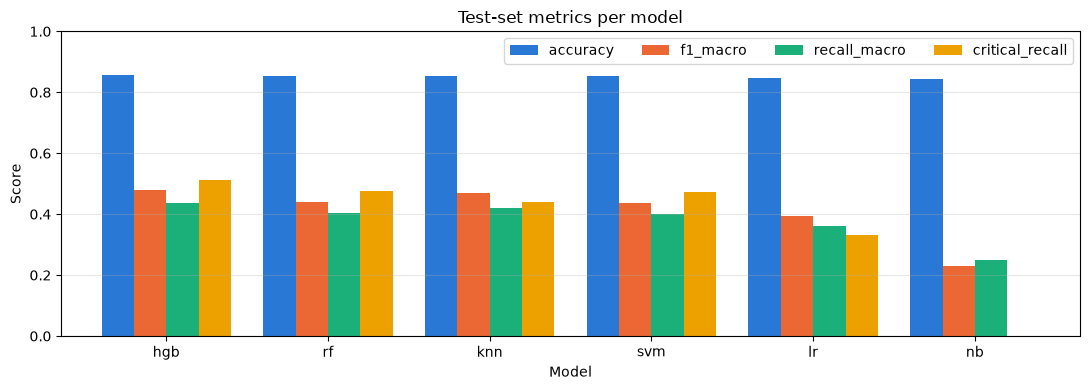
\includegraphics[width=0.95\textwidth]{test_metrics}
\caption{Test-set metrics per model. Accuracy is nearly flat across models; the imbalance-aware
metrics are what distinguish them.}
\label{fig:metrics}
\end{figure}

Three observations stand out:

\begin{itemize}[itemsep=3pt]
  \item \textbf{Gradient boosting wins on every metric.} It is the only model that improves
        on the majority-class baseline by more than 1.4 accuracy points while also reaching the
        best macro-F1 and the best Critical recall (51\,\%).
  \item \textbf{Naive Bayes degenerates to the majority class.} Its accuracy equals the share of
        Low encounters exactly (0.8423) and it never predicts any other class. The selected
        variance smoothing of $1.0$, the largest value in the grid, effectively flattens all
        likelihoods; the strong correlations between features (counts of visits, procedures and
        medications grow together) violate the conditional-independence assumption.
  \item \textbf{KNN is a surprisingly strong second on macro-F1}, ahead of random forest and
        SVM, because it recovers more Medium encounters (recall 0.14 versus 0.03--0.05). It pays
        for it with the slowest prediction after SVM.
\end{itemize}

\subsection{Per-class behaviour}

Figure~\ref{fig:perclass} and Table~\ref{tab:perclass} break the best model down by class, and
Figure~\ref{fig:cmall} shows the confusion matrices of all six models.

\begin{figure}[H]
\centering
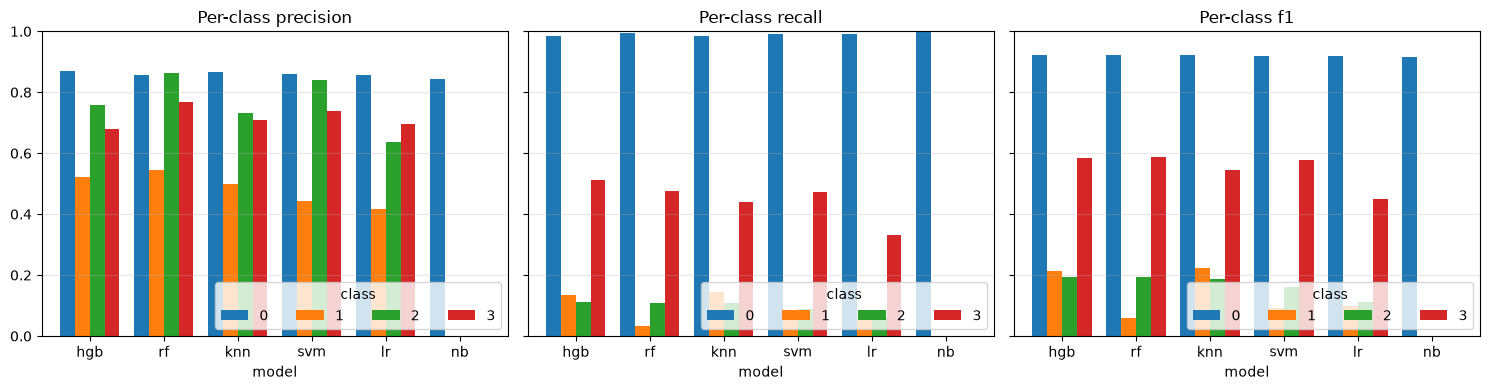
\includegraphics[width=\textwidth]{per_class}
\caption{Per-class precision, recall and F1 on the test set for every model.}
\label{fig:perclass}
\end{figure}

\begin{table}[H]
\centering\small
\caption{Per-class report of the best model (histogram gradient boosting) on the test set.}
\label{tab:perclass}
\begin{tabular}{@{}lrrrr@{}}
\toprule
\textbf{Class} & \textbf{Precision} & \textbf{Recall} & \textbf{F1} & \textbf{Support} \\
\midrule
0 -- Low      & 0.868 & 0.985 & 0.923 & 17{,}384 \\
1 -- Medium   & 0.522 & 0.135 & 0.215 &  2{,}037 \\
2 -- High     & 0.760 & 0.111 & 0.194 &    879 \\
3 -- Critical & 0.678 & 0.512 & 0.583 &    338 \\
\midrule
Macro average    & 0.707 & 0.436 & 0.479 & 20{,}638 \\
Weighted average & 0.826 & 0.857 & 0.817 & 20{,}638 \\
\bottomrule
\end{tabular}
\end{table}

\begin{table}[H]
\centering\small
\caption{Confusion matrix of the best model on the test set (rows: true class, columns: predicted class).}
\label{tab:cm}
\begin{tabular}{@{}l|rrrr@{}}
\toprule
\textbf{True} $\backslash$ \textbf{Pred.} & \textbf{Low} & \textbf{Medium} & \textbf{High} & \textbf{Critical} \\
\midrule
Low      & \best{17{,}131} &  189 &   4 &  60 \\
Medium   &  1{,}726 & \best{275} &  25 &  11 \\
High     &    713 &   57 & \best{98} &  11 \\
Critical &    157 &    6 &   2 & \best{173} \\
\bottomrule
\end{tabular}
\end{table}

\begin{figure}[H]
\centering
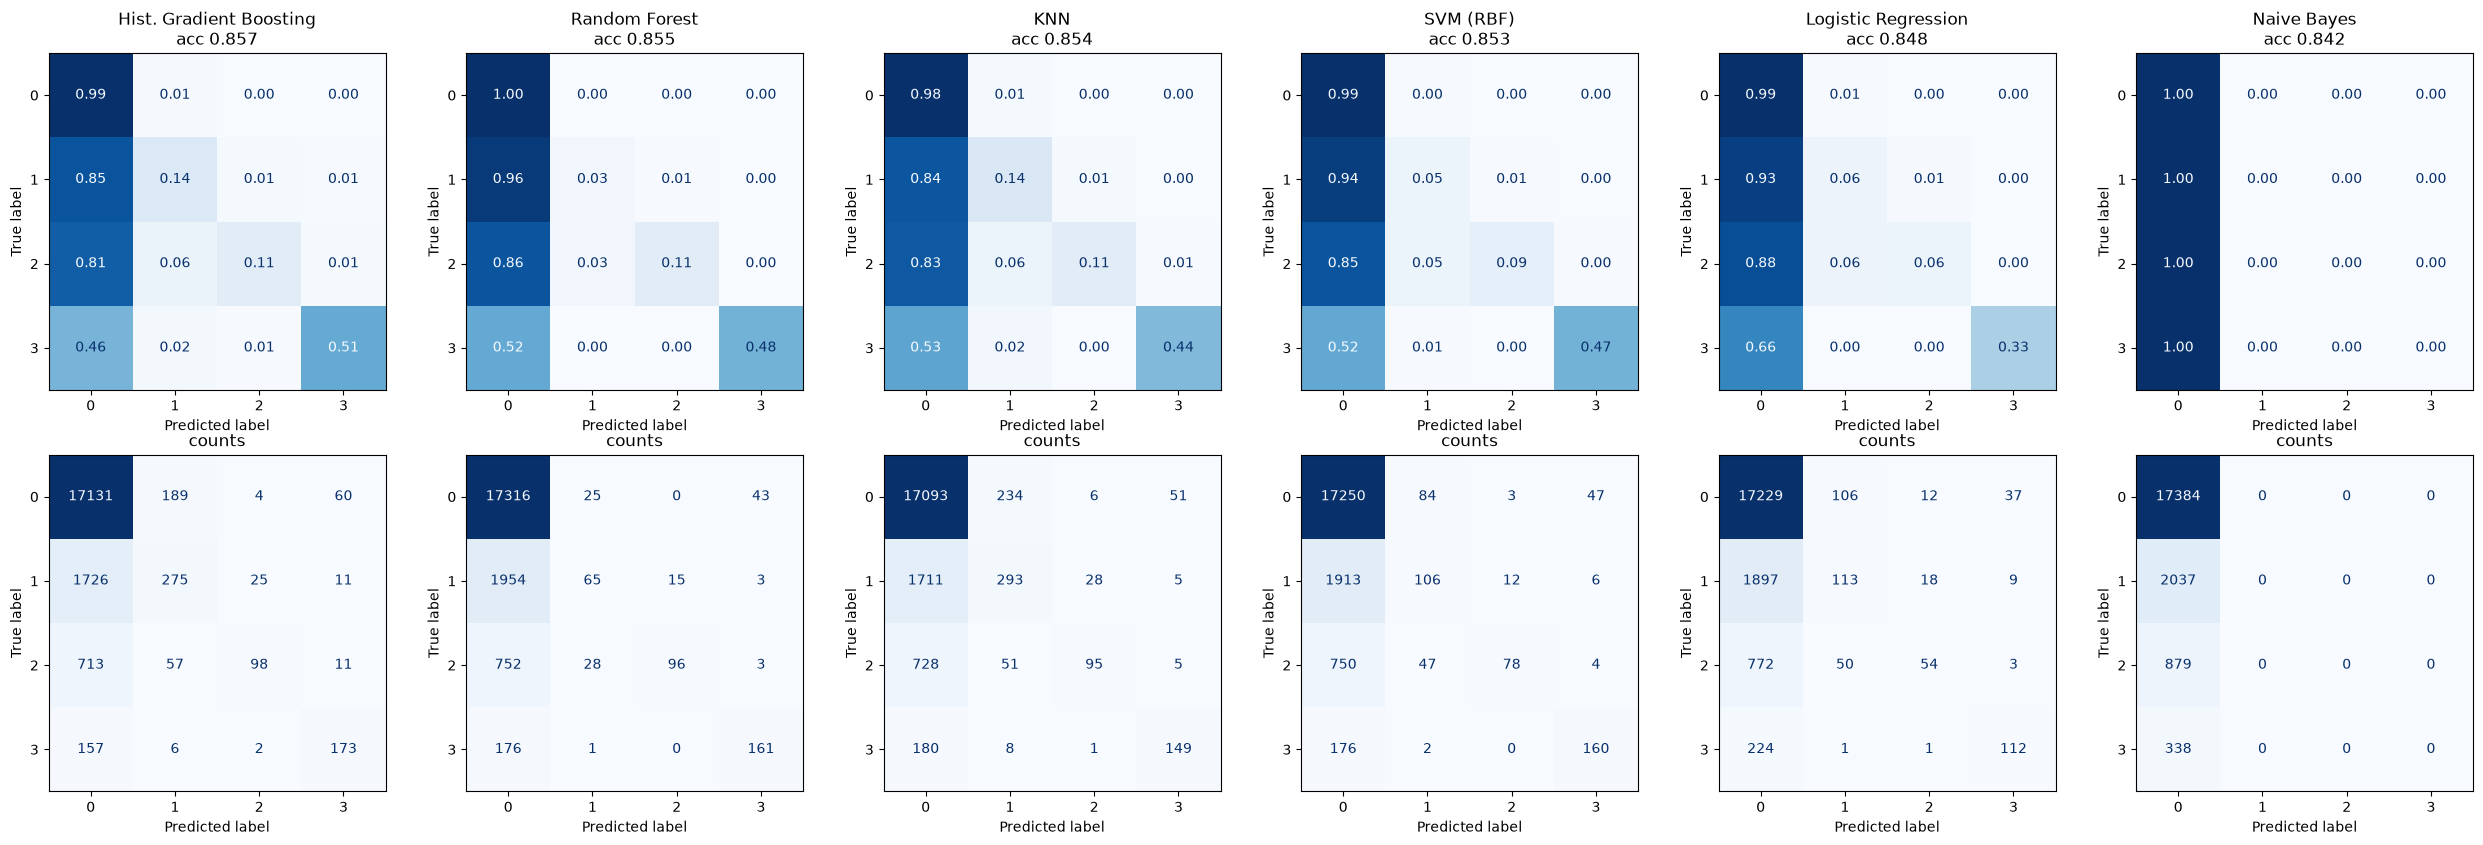
\includegraphics[width=\textwidth]{confusion_all}
\caption{Row-normalised confusion matrices (top; the diagonal is the per-class recall) and raw
counts (bottom) for the six models, ordered by test accuracy.}
\label{fig:cmall}
\end{figure}

\begin{figure}[H]
\centering
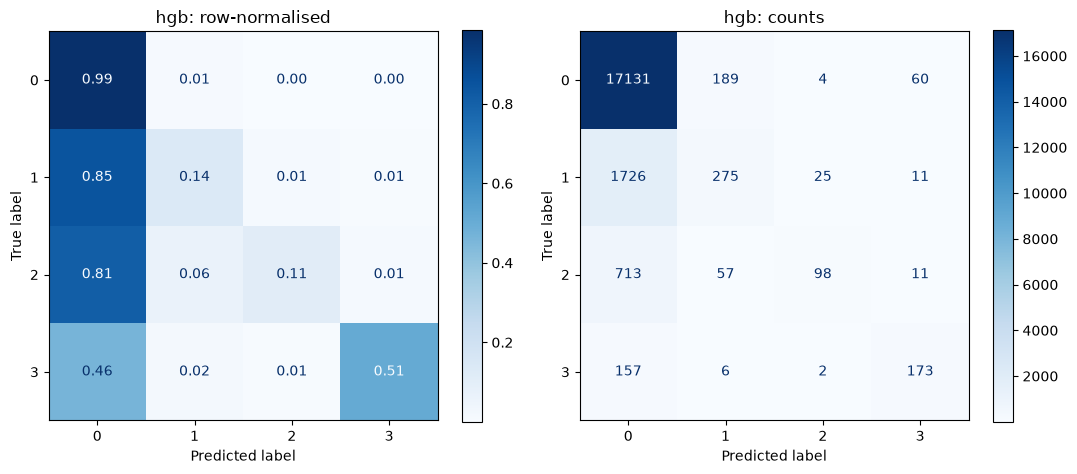
\includegraphics[width=0.9\textwidth]{confusion_best}
\caption{Confusion matrix of histogram gradient boosting, the best model.}
\label{fig:cmbest}
\end{figure}

The matrices tell a consistent story. The \textbf{Low} class is recognised almost perfectly
(recall 0.98--1.00). The \textbf{Critical} class is the second easiest: about half of the Critical
encounters are caught by the tree ensembles, the SVM and KNN, with a precision around 0.7. These
encounters correspond to inpatient or emergency visits followed by death within 30 days, and the
patients concerned usually have a long and heavy history (many prior urgent visits, chronic
kidney disease, cancer), which the models pick up.

The \textbf{Medium} and \textbf{High} classes are where every model fails: at most 14\,\% of
Medium and 11\,\% of High encounters are recovered, and almost all the rest are predicted Low.
This is expected from the way the label was built. A Medium or High encounter is typically an
urgent-care or emergency visit, whose occurrence depends on an acute event (an injury, an
infection) that the patient's prior history cannot foresee. The features describe the chronic
background, not the trigger of the visit.

\subsection{Which features matter}

As a sanity check, the impurity-based feature importances of the fitted random forest were
inspected (Table~\ref{tab:importance}). The dominant signals are exactly the ones a clinician
would expect: how often the patient has already needed urgent care, kidney function (glomerular
filtration rate and the chronic kidney disease flag), the overall density of the medical history
and age.

\begin{table}[H]
\centering\small
\caption{Ten most important features of the random forest (mean decrease in impurity).}
\label{tab:importance}
\begin{tabular}{@{}llr@{}}
\toprule
\textbf{Rank} & \textbf{Feature} & \textbf{Importance} \\
\midrule
1  & Prior urgent visits & 0.098 \\
2  & Glomerular filtration rate (MDRD) & 0.081 \\
3  & Prior visits & 0.058 \\
4  & Prior imaging studies & 0.058 \\
5  & Prior conditions & 0.057 \\
6  & Chronic kidney disease flag & 0.046 \\
7  & Prior medications & 0.041 \\
8  & Age (years) & 0.038 \\
9  & Cancer flag & 0.036 \\
10 & QALY & 0.033 \\
\bottomrule
\end{tabular}
\end{table}

% =====================================================================
\sect{Discussion}
\label{sec:discussion}
% =====================================================================

\paragraph{The choice of tuning metric is a policy decision.}
All searches recorded four metrics but selected on accuracy, and every winning configuration
ended up with \emph{no} class weighting. The training notebook documents the alternative that was
explored: selecting on macro-recall instead pushes every model to \code{class\_weight="balanced"},
raising Critical recall to roughly 0.8 at the price of an accuracy drop to about 0.6, because many
Low encounters are then flagged as risky. Neither extreme is ``right''; macro-F1 is the natural
compromise and is the metric the notebook recommends. For a deployment in triage, the cost of a
missed Critical patient is much higher than that of a false alarm, so a recall-oriented choice
would probably be preferred.

\paragraph{The label is a heuristic.}
The risk score of Equation~\eqref{eq:score} is a reasonable proxy for visit severity, but it is
hand-crafted. In particular, the base severity of the encounter class dominates the score, so the
classification task is close to ``predict the type of the next visit from the past''. The 0.25
and 0.50 thresholds also split visit types rather sharply: the Low/Medium boundary essentially
separates routine visits from urgent-care ones.

\paragraph{Synthetic data.}
Synthea histories are generated by disease-progression modules; they are internally consistent but
smoother and more regular than real records. Results should be read as a validation of the
pipeline rather than as clinical performance figures.

\paragraph{Computational trade-offs.}
Tuning on a 20{,}000-row subsample with 3 folds kept the complete training run around six
minutes. The SVM was the bottleneck (195 s of search plus 51 s for a final fit limited to
40{,}000 rows, and 14 s to predict the test set) while delivering no advantage over gradient
boosting, which tunes in 12 s and predicts in 0.3 s.

% =====================================================================
\sect{Final model choice}
\label{sec:choice}
% =====================================================================

The model retained for the project is the \textbf{histogram-based gradient boosting classifier}
(learning rate 0.03, 400 boosting iterations, 31 leaves, minimum 20 samples per leaf,
$\ell_2$ regularisation 0.1), implemented in scikit-learn by the class
\code{HistGradientBoostingClassifier}. The decision rests on four arguments, summarised in
Table~\ref{tab:choice}.

\begin{table}[H]
\centering\small
\caption{Decision matrix for the final model. Ranks are out of six (1 is best).}
\label{tab:choice}
\begin{tabular}{@{}lccccc@{}}
\toprule
\textbf{Model} & \textbf{Accuracy} & \textbf{Macro-F1} & \textbf{Critical recall} & \textbf{Train + predict} & \textbf{Overall} \\
\midrule
Hist.\ gradient boosting & 1 & 1 & 1 & fast (18 s / 0.3 s) & \best{selected} \\
Random forest            & 2 & 3 & 2 & fast (79 s / 0.1 s) & runner-up \\
KNN                      & 3 & 2 & 4 & slow predict (1.5 s) & -- \\
SVM (RBF)                & 4 & 4 & 3 & slow (246 s / 14 s) & -- \\
Logistic regression      & 5 & 5 & 5 & very fast & -- \\
Naive Bayes              & 6 & 6 & 6 & very fast & degenerate \\
\bottomrule
\end{tabular}
\end{table}

\paragraph{1. It is the best model on every metric, not just one.}
Gradient boosting ranks first on accuracy (0.857), macro-F1 (0.479), macro-recall (0.436) and
Critical recall (0.512). The other candidates each trade one quality for another: random forest is
close on accuracy but recovers only 3\,\% of Medium encounters, KNN is close on macro-F1 but misses
more Critical patients, and the SVM is never better than the forest. Choosing on a single metric
could be contested; a model that dominates on all four cannot.

\paragraph{2. It handles the structure of the data.}
The features mix counts with heavy tails (up to 15{,}289 prior imaging studies), binary flags and
lab values on very different scales, and many of them are strongly correlated (the history counts
grow together with age). Tree-based boosting is invariant to feature scaling, models non-linear
thresholds (for instance a sharp drop in glomerular filtration rate) and interactions between
features natively, and is robust to correlated inputs. This explains why both tree ensembles beat
the distance-based and linear models, and why Naive Bayes, which assumes independent Gaussian
features, collapsed entirely.

\paragraph{3. It is cheap to train, tune and serve.}
The full search of 20 configurations took 12 s and the final fit on 82{,}551 rows 6 s. Scoring the
whole test set takes 0.3 s, i.e.\ about 15 microseconds per encounter, which is compatible with
real-time use at admission. By contrast the SVM needed more than four minutes of search, had to be
fitted on a reduced training set, and is 40 times slower at prediction for a worse result.

\paragraph{4. It is the easiest model to improve further.}
The model exposes calibrated class probabilities, so the decision threshold for the Critical class
can be lowered to favour recall without retraining (Section~\ref{sec:discussion}). It also accepts
\code{class\_weight="balanced"} and supports SHAP explanations, which are the three most
promising next steps. None of the other competitive models (KNN, SVM) offers the same combination.

\paragraph{Honest limits of the choice.}
The margin over random forest is small on accuracy (0.2 points) and the two models are
interchangeable for the Low and Critical classes; the difference lies in the Medium class, where
boosting recovers four times more encounters. The selection was also made on accuracy-tuned
configurations; had the search optimised macro-F1 or recall, the ranking might shift, although
boosting also led the cross-validation on macro-F1 (0.432 versus 0.408 for the forest).

% =====================================================================
\sect{Conclusion and future work}
% =====================================================================

Starting from twelve Synthea tables, this project built a leakage-free encounter-level dataset of
103{,}189 samples and 55 numeric features, defined a four-level risk label, and compared six
classifiers under a reproducible protocol. Histogram-based gradient boosting is the best model on
every metric, with a test accuracy of 0.857, a macro-F1 of 0.479 and a Critical recall of 0.51,
and it is also among the cheapest to train and to run. The remaining weakness is the Medium and
High classes, which the prior history alone does not predict well.

Several directions could improve on this baseline:

\begin{itemize}[itemsep=2pt]
  \item \textbf{Re-tune on macro-F1 or a cost-sensitive objective}, and apply
        \code{class\_weight="balanced"} or resampling (SMOTE, undersampling of Low), to trade a
        little accuracy for far better recall on the rare classes.
  \item \textbf{Threshold tuning on predicted probabilities} instead of the arg-max decision,
        which allows the Critical sensitivity to be set explicitly.
  \item \textbf{Richer temporal features}: time since the last urgent visit, trends in vitals,
        number of visits in the last 30/90/365 days rather than lifetime counts.
  \item \textbf{Alternative formulations}: regress the continuous \code{risk\_score} directly, or
        merge Medium and High into a single ``elevated'' class.
  \item \textbf{Model explainability}: SHAP values on the gradient boosting model to explain
        individual Critical predictions to clinicians.
\end{itemize}

% =====================================================================
\appendix
\sect{Full feature list after preprocessing}
\label{app:features}
% =====================================================================

\begin{table}[H]
\centering\small
\caption{The 55 features used by every model.}
\begin{tabular}{@{}lp{10.6cm}@{}}
\toprule
\textbf{Family} & \textbf{Columns} \\
\midrule
Demographics (7) &
  \code{age\_years}, \code{age\_months}, \code{INCOME}, \code{gender\_m}, \code{gender\_f},
  \code{race}, \code{is\_hispanic} \\
\addlinespace
History counts (10) &
  \code{prior\_visits}, \code{prior\_urgent\_visits}, \code{prior\_conditions},
  \code{prior\_medications}, \code{prior\_procedures}, \code{prior\_immunizations},
  \code{prior\_allergies}, \code{prior\_careplans}, \code{prior\_imaging\_studies},
  \code{prior\_devices} \\
\addlinespace
Risk-factor flags (10) &
  \code{rf\_hypertension}, \code{rf\_diabetes}, \code{rf\_heart\_disease}, \code{rf\_copd},
  \code{rf\_obesity}, \code{rf\_smoker}, \code{rf\_stroke}, \code{rf\_ckd}, \code{rf\_cancer},
  \code{rf\_asthma} \\
\addlinespace
Observations (28), prefix \code{obs\_} &
  \emph{Vitals and body:} body height, body weight, BMI ratio, systolic and diastolic blood
  pressure, heart rate, respiratory rate, pain severity (0--10). \newline
  \emph{Blood chemistry:} glucose, calcium, sodium, potassium, chloride, total carbon dioxide,
  creatinine, urea nitrogen, glomerular filtration rate (MDRD), hemoglobin A1c. \newline
  \emph{Lipid panel:} total cholesterol, HDL, LDL, triglycerides. \newline
  \emph{Questionnaires and quality of life:} PHQ-2, GAD-7, QOLS, QALY, DALY, household size. \\
\bottomrule
\end{tabular}
\end{table}

\sect{Reproducibility}

\begin{itemize}[itemsep=2pt]
  \item \textbf{Environment}: Python 3.14, pandas 3.1, scikit-learn 1.9, matplotlib 3.11,
        joblib 1.6 (managed with Poetry).
  \item \textbf{Seed}: 156\,543\,894 for the train/test split, the tuning subsample, the CV folds,
        the randomised searches and the tree ensembles.
  \item \textbf{Artefacts}, all stored in \code{prediction/ml/models/}: the six fitted models
        (\code{*\_model.joblib}), the selected hyper-parameters (\code{best\_params.json})
        and the test indices (\code{split.json}).
  \item \textbf{Order of execution}: \code{build\_dataset.py} $\rightarrow$
        \code{preprocessing.ipynb} $\rightarrow$ \code{training.ipynb} $\rightarrow$
        \code{evaluation.ipynb}.
\end{itemize}

\end{document}
